\section{Tracking performance}\label{sec:tracking}
\sectionstate{partial}{angle: \texttt{papers/paper1\_v2/figs/make\_angle\_resolution\_v2.py} and \texttt{out/angle\_resolution\_v2.json}
(same selection and statistic as \texttt{rerun/paper1\_res/angle\_resolution.py}); reference term \texttt{rerun/model\_audit/followups/gb\_m3\_angle};
budget \texttt{rerun/paper1\_floor/README.md}; position \texttt{rerun/paper1\_floor}, \texttt{rerun/sps\_region}; time and gain
\texttt{figs/make\_gain\_scan.py}, \texttt{out/gain\_scan.json}, \texttt{rerun/paper1\_timing}. v2 2026-11-10: this is the old
section 7.1--7.4 with the timing section and the gain paragraphs of the old section 5.3 joined to it; the angle subsection is
written out (it was 50 words).}
\intent{What one chamber delivers on a single track: the angle, which is the figure of merit, then position and time,
and how little of it depends on the gain.}

\subsection{Angular resolution}\label{sec:angle}
The angle is measured against the reference track on cosmic muons, in the interior of the chamber
(\cref{sec:definitions}). \Cref{fig:angle} gives the result for chamber~A: over Runs 1 and 2, 25\,400 matched single
tracks per view, the resolution is
\[ s_{68}=0.99^\circ\ \text{(X)}\qquad\text{and}\qquad 0.90^\circ\ \text{(Y)}, \]
with a median residual below 0.02\textdegree. Four properties of this number matter.

\emph{It is the chamber's own.} The reference angle is far better than the chamber's. The telescope and the multiple
scattering of the muons between its planes contribute about 0.05\textdegree, and the data bound that contribution at
0.11\textdegree{} in X and 0.14\textdegree{} in Y; in quadrature with one degree that is under one per cent.
\askDylan{The 0.11/0.14\textdegree{} bound is from the two-chamber position pin of chambers C and D (26 June); for chamber~A
alone a kink regression gives ${\le}0.055$\textdegree. The material of the bench was never recorded. Say which bound you want
quoted.}

\emph{It holds out of sample.} The calibration was made on Run~1. Run~1 gives $0.98^\circ$ and $0.90^\circ$; Run~2,
which the calibration never saw, gives $0.99^\circ$ and $0.90^\circ$.

\emph{It does not depend on the angle.} Across the $\pm20$\textdegree{} that the bench provides, the resolution stays
within about 0.15\textdegree{} of its mean (\crefp{fig:angle}{b}). In the beam, with chamber~E yawed by
25.4\textdegree{}, the angle scale is $0.98\pm0.03$ of the known angle~\cite{paperII}, so the scale holds beyond the
reach of the bench.
\analysis{SPS25}{a resolution at 25\textdegree{} with the beam as reference is not quoted: the two existing numbers (0.96--0.99\textdegree{} on an
older fit, 1.02--1.10\textdegree{} on the final one) clip at 5\textdegree{} with 20\,\% of tracks beyond 10\textdegree. A clean one needs a single-track
selection and unclipped $s_{68}$ on the CF$_4$ runs that have a column-measured $\vd$; those runs exist.}

\emph{It includes one correction.} The readout boards are bowed, which tilts the drift direction by an amount that
varies across the chamber (\cref{sec:bow}). The correction is part of the calibration. Without it chamber~A reads
1.10\textdegree{} and 1.07\textdegree.

The residual is not Gaussian (\crefp{fig:angle}{a}). Beyond its core lies a flat floor: 3.4\,\% of tracks in each
view are more than 5\textdegree{} off, and these are fits far steeper than the track, not a wider core. They are the
events of \cref{sec:straight}, in which a $\delta$-ray or a second deposit pulls a straight-line fit.

Chamber~B, the second good chamber, reaches $1.05^\circ$ and $1.13^\circ$, also flat in angle
(\crefp{fig:angle}{b}). Chambers C, D and E reach $1.26/1.51^\circ$, $1.23/1.46^\circ$ and $2.41/2.08^\circ$
(\crefp{fig:angle}{c}); these three were calibrated on the runs they are quoted on, and they are the chambers with
production defects (\cref{sec:conclusions}).

\paragraph{What it is compared with.} A conventional micro-TPC analysis fits a straight line to one time per strip.
On the same chamber~A events and with one statistic for both, that gives 2.1\textdegree{} and 2.7\textdegree{} where
the waveform fit gives 1.0\textdegree~\cite{paperII}. A simulation of the reconstruction on ideal events gives
0.3--0.5\textdegree, so the chamber is a factor of two above what its geometry and sampling allow. Part of the
excess is in events with saturated strips or unusually large charge. The rest behaves as an event-to-event
fluctuation of the charge pattern that is larger in the data than in the simulation; it is characterised in the
companion paper and its origin in the signal is not identified.
\askDylan{This replaces ``an unexplained remainder of 0.56--0.65\textdegree{} on clean events is measured and bounded but not
identified''. That number is on another footing from the headline ($s_{68}$ within $\pm5$\textdegree, calibration runs, a
different arm), so it is not quoted here; give it in the companion paper with its definition, or tell me to put it back.
The 2.1/2.7\textdegree{} against 1.0\textdegree{} comparison is in the companion paper's convention too (clip at 5\textdegree, no bow
correction: 1.04/1.01\textdegree), which is why it is not drawn in \cref{fig:angle}.}

\begin{figure}[tbp]
  \centering
  \figorbox{angle_resolution_v2}{residual distribution, resolution against angle for A and B, all chambers}
  \caption{Angular resolution on cosmic muons. (a) The residual $\theta_\mathrm{fit}-\theta_\mathrm{ref}$ of
  chamber~A (Runs 1 and 2, 25\,400 reference-matched single tracks per view), X filled and Y open, per degree on a
  logarithmic scale; vertical lines, the median $\pm\,s_{68}$. Beyond $\pm15$\textdegree{} lie 2.5\,\% (X) and 2.6\,\% (Y)
  of the tracks. (b) $s_{68}$ in 2\textdegree{} bins of the reference angle for chambers A and B, X solid and Y dashed;
  bootstrap errors. (c) $s_{68}$ of each chamber in its interior, X filled and Y open. $s_{68}$ is the 68th percentile of
  $|\theta_\mathrm{fit}-\theta_\mathrm{ref}-\mathrm{median}|$, with no clipping.}
  \label{fig:angle}
\end{figure}

\subsection{What the resolution means at the target}\label{sec:pointing}
With \cref{eq:pointing}, a track measured to 0.99\textdegree{} (0.90\textdegree) points back to the target, 233\,mm
away, to 4.0\,mm (3.7\,mm), and the position resolution of the next subsection contributes 0.1\,\% of that variance.
For the leptons the chambers were built for, the multiple scattering in the air and in the entrance foils of the
chamber is larger than this at every energy: 4.5\,mm at 16\,MeV, 8.8\,mm at 8\,MeV and 17\,mm at 4\,MeV
(\cref{tab:material}, \crefp{fig:pointing}{b}). The chamber therefore meets the requirement of \cref{sec:requirement}:
its own resolution is not what limits the pointing. Nor does it limit the opening angle of a pair, which the two
chambers alone would give to 1.3\textdegree{} and the scattering of two 10\,MeV leptons brings to 3.6\textdegree{}
(\cref{sec:requirement}). The foils are worth attention for the same reason. The copper of
the cathode alone, if it is the 9\,\textmu m assumed here, scatters as much as the 20\,cm of air.

\subsection{Position resolution}\label{sec:position}
The residual of the reconstructed position to the reference ray at the mesh has a Gaussian core of 0.55\,mm in X and
0.53\,mm in Y for chamber~A. Little of that is the chamber. The residual holds three terms: the chamber, the pointing
of the reference ray (0.24 and 0.21\,mm), and the scattering of the muon between the reference planes, which shows as
a growth of the residual with the $\chi^2$ of the reference track. Extrapolating the core width of tracks near normal
incidence to $\chi^2\to0$ removes the scattering (\crefp{fig:posres}{a}) and leaves $275\pm15$ and
$236\pm18$\,\textmu m; subtracting the pointing in quadrature leaves the chamber, $128\pm33$\,\textmu m in X and
$113\pm36$\,\textmu m in Y. The subtraction dominates the uncertainty: a change of 10\,\% in the pointing moves these to
63--166 and 62--145\,\textmu m (\crefp{fig:posres}{b}). We quote an intrinsic resolution of about
$120\pm60$\,\textmu m for chamber~A near normal incidence. Chamber~B gives $163\pm29$ and $176\pm21$\,\textmu m.

The beam gives an independent check with another reference. In its working region (\cref{app:beam}), chamber~E
measures $138$\,\textmu m in X and $120$\,\textmu m in Y after the pointing of the telescope is subtracted, with
ranges of 112--153 and 89--136\,\textmu m from the uncertainty of the telescope and upper bounds of 153 and
145\,\textmu m that assume nothing about it (\crefp{fig:posres}{c--e}). Chamber~E runs at reduced gain over most of
its board, so this is a cross-check and not the headline; the two setups agree.

\begin{figure}[tbp]
  \centering
  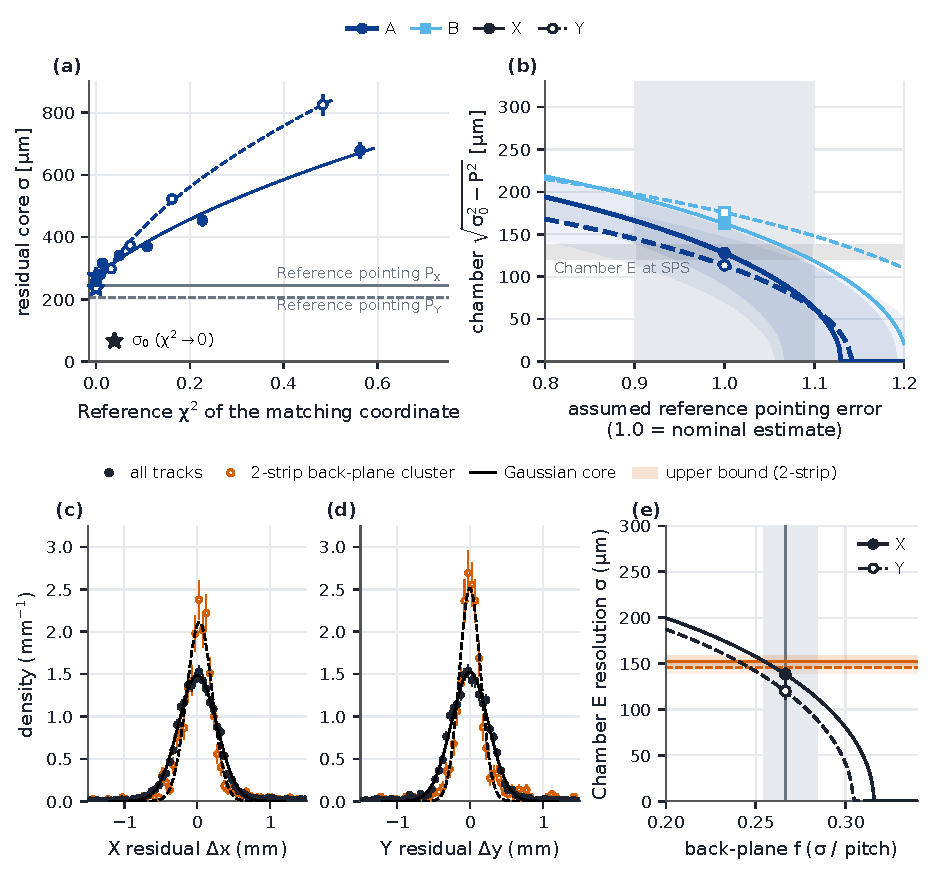
\includegraphics[width=0.9\linewidth]{position_res}
  \caption{Position resolution. Top, bench: (a) core width of the chamber~A residual for tracks within 5\textdegree{}
  of normal incidence, against the mean $\chi^2$ of the reference track in the matching coordinate, with $\sigma^2$
  linear in $\chi^2$ extrapolated to $\chi^2\to0$ (stars); horizontal lines, the pointing of the reference ray. (b) The
  chamber term, the extrapolated width less the pointing in quadrature, against the pointing error assumed, in units of
  its nominal estimate, for chambers A and B (X solid, Y dashed); the vertical band is $\pm10$\,\% on the pointing, the
  horizontal band chamber~E in the beam. Bottom, beam, chamber~E in its working region: (c) X and (d) Y residuals to
  the telescope for all tracks and for tracks with a two-strip cluster in the back plane of the telescope, with
  Gaussian cores; (e) the resolution of chamber~E after subtracting the telescope against the resolution assumed for
  that back plane in units of its pitch (shaded: its measured value), with the upper bounds that assume none.}
  \label{fig:posres}
\end{figure}

\subsection{Time resolution}\label{sec:time}
The reconstruction returns the time at which the charge of a track starts to arrive, in each view. Against the
scintillator trigger, the event time of chamber~A has a resolution of 41.6\,ns in Run~1 and 40.3\,ns in Run~2. The
difference between the two views, which cancels everything they share, gives 22.4 and 22.2\,ns for
$(t_X-t_Y)/\sqrt2$, the part of the resolution that is uncorrelated between the views; what the two views share is 38
and 37\,ns. In a TPC time is depth: at 36\,\textmu m/ns the event time is 1.5\,mm along the drift. Chambers B and D
reach 42 and 46\,ns, chamber~C 78\,ns (\cref{app:gain}).

The time resolution is set by the size of the signal, as the next subsection shows, and a correction for time walk
changes it by less than 1\,\%. The dependence on the drift field is in \cref{app:gain}.

\subsection{What the gain buys: time, and nothing else}\label{sec:gain}
Chamber~A was scanned in $HV_\mathrm{resist}$ from 425 to 525\,V at fixed drift field (\cref{fig:gainscan}). Between
425 and 490\,V the charge of a track grows by a factor $13.1\pm0.5$, doubling every $17.5\pm0.3$\,V on average (every
19\,V at the bottom of the range and every 15\,V at the top), and the fraction of tracks with a strip at the limit of
the ADC rises from zero to 30\,\%.

Over that factor of 13 the angular resolution does not move: 0.91--1.03\textdegree{} in X and 0.80--0.96\textdegree{}
in Y up to 505\,V, with an angle scale of 0.99--1.02 in both views (\crefp{fig:gainscan}{b}). Nor does the core of the
position residual (\crefp{fig:gainscan}{c}), nor the efficiency (\cref{sec:hvscan}). The time resolution does: the
uncorrelated part falls from $83\pm10$\,ns at 425\,V to $24\pm1$\,ns at 490\,V, and the event time from $102\pm8$ to
$38\pm2$\,ns (\crefp{fig:gainscan}{d}).

The reason is that the two come from different parts of the signal. The time is read from the start of the charge
column, the first electrons, made next to the mesh: a small part of the signal, whose timing degrades as it nears the
noise. The angle is fitted to the whole column, every strip and every sample. Two measurements support this. Track
by track, among unsaturated tracks of the scan points below 510\,V, the angle residual does not depend on the charge
of the track over a factor 17 in charge. And in a fixed window of early amplitude the uncorrelated time changes only
from $44\pm5$\,ns at 435\,V to $30\pm4$\,ns at 490\,V, against a factor of about four over the same voltages for all
signal sizes: most of its dependence on the voltage is the size of the signal. The event time in the same window still falls, from $82\pm8$ to $39\pm4$\,ns, so
the part common to the two views has a dependence on the voltage that the amplitude does not account for.
\askDylan{Three corrections from the HV rundown (\texttt{figs/out/gain\_scan.json}): (1) the time values against HV are now
those of reference-matched tracks, as everywhere else in the paper (83/102\,ns at 425\,V); the old text and one appendix
figure used all clean triggers, 80\,\% of which have no reference track (109/105\,ns). (2) The gain: one doubling voltage
does not describe the curve; 16.7\,V came from a fit pulled by the long run and 18.8\,V from the bottom of the range. (3)
``At fixed amplitude the HV barely matters'' holds for the uncorrelated part only (and a constant is disfavoured at
2.6$\sigma$ even there); the event time still falls. The old claim that the common part ``does not fall'' is about the drift
field (\cref{app:gain}), not the voltage. The angle-by-charge-decile numbers (0.82--0.94\textdegree{} X, 0.72--0.87\textdegree{} Y) have
no producer in the repo, so they are not quoted; the sentence ``does not depend on the charge of the track over a factor
17'' rests on the same missing script and needs re-deriving or dropping. The fixed-window numbers are on all clean
triggers, not on reference-matched tracks.}
Two limits apply. The angular resolution includes the small reference term, which could hide a change in the
chamber's own; and the statement holds down to 425\,V, $1/13$ of the gain of the long runs, below which the scan does
not go. For operation the consequence is margin: the chamber could run well below 490\,V with no loss of efficiency,
angle or position, at the price of the time resolution.
\askDylan{The bench runs used 490\,V; the scans support any HV from ${\sim}460$\,V up for efficiency. Is timing
(depth, $t_0$) the argument we want to make for 490\,V, or was it chosen for gain margin at n\_TOF? Note the noise floor
doubled there (23 July), which would favour margin, but we have no n\_TOF HV scan to show it.}

\begin{figure}[tbp]
  \centering
  \figorbox[width=0.88\linewidth]{gain_scan}{chamber A against the resist HV: charge and saturation, angle, position, time}
  \caption{Chamber~A against $HV_\mathrm{resist}$ (scan of 27 June at 1000\,V on the cathode). (a) Track charge, the
  25th percentile with saturated tracks ranked above all others (diamonds, logarithmic scale; dotted, an exponential
  fitted from 425 to 495\,V) and, right axis, the fraction of tracks with a saturated strip (stars). (b) Angular
  resolution $s_{68}$ and, right axis, the angle scale (the slope of the fitted against the reference $\tan\theta$).
  (c) Core of the position residual at the mesh, reference pointing and scattering included. (d) Time resolution of
  reference-matched tracks: event time (filled) and the uncorrelated part $(t_X-t_Y)/\sqrt2$ (open). X filled and solid,
  Y open and dashed. Dotted vertical line: 490\,V, the voltage of Runs 1 and 2.}
  \label{fig:gainscan}
\end{figure}
